%% This is an example first chapter.  You should put chapter/appendix that you
%% write into a separate file, and add a line \include{yourfilename} to
%% main.tex, where `yourfilename.tex' is the name of the chapter/appendix file.
%% You can process specific files by typing their names in at the 
%% \files=
%% prompt when you run the file main.tex through LaTeX.
\chapter{Evolutionäre Algorithmen}

Diese Subkategorie von Algorithmen wurde durch den natürlichen Prozess der Evolution
inspiriert. Charles Darwin begründete 1838 den Evolutionsprozess und das daraus resultierende
Überleben der jeweils am besten angepassten Individuen mit der natürlichen Selektion.
Diese stellt sicher, dass sich gut an den Lebensraum angepasst Lebewesen in der Natur
durchsetzen können, währenddessen weniger gut angepasste Individuen aussterben. Zudem
arbeitet die Natur nach dem 'Trial and Error' Prinzip. Dadurch werden Mutationen an
Lebewesen ausprobiert und bei positivem Effekt auf das Überleben der Spezies beibehalten,
bei einer Verminderung der Überlebenschancen jedoch wieder rückgängig gemacht. Dieser Prozess
ist sehr zeitaufwändig, jedoch nachhaltig wirksam. Viele Algorithmen wie beispielsweise
der Hill Climbing Algorithmus wenden ebenfalls dieses Prinzip an.

\section{Anwendungsgebiete}
hier anwendungsfälle definieren

\section{Genetische Algorithmen}

Die Genetischen Algorithmen sind die bekanntesten Vertreter aus der Gruppe der Evolutionären
Algorithmen. Sie orientierten sich an der Populationsgenetik und insbesondere an den Mendelschen
Regeln. \cite{Mcc00}
Bei Genetischen Algorithmen werden häufig Begriffe aus der Biologie verwendet. Die Anzahl an
möglichen Lösungen nennt man Population. Eine einzelne Lösungsvariante wird als Chromosom
bezeichnet, wohingegen diese wiederum aus einer Kombination an Variablen, in der Biologie Gene
genannt, bestehen. Wie aus der Grafik \ref{fig:genetics} zu entnehmen ist, besteht ein Chromosom
$A_n$ aus mehreren Genen.
\\
\begin{figure}[h!]
  \centering
  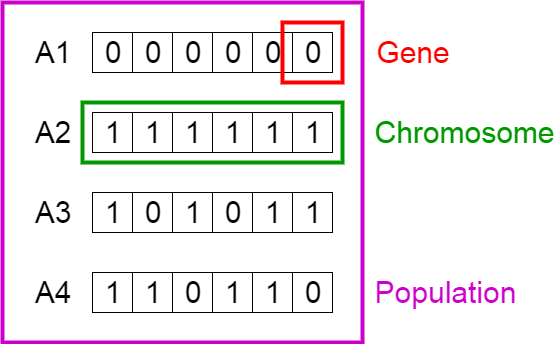
\includegraphics[scale=0.6]{resources/genetic_algorithms.png}
  \caption{Population, Chromosome und Gene}
  \label{fig:genetics}
\end{figure}

Im folgenden werden die einzelnen Schritte erläutert, welche die Natur wie auch die Genetischen
Algorithmen durchlaufen, um eine Anfangspopulation schrittweise weiterzuentwickeln. Die Natur
sucht nach der erfolgsversprechendsten Lösung zum Überleben, wohingegen die Algorithmen
optimale Lösungen für ganz unterschiedliche Problemstellungen suchen. \cite{Mal17}

\subsection{Initiale Population}
Eine Population besteht aus mehreren unabhängigen Lösungen, im biologischen Kontext Chromosomen,
um eine bestimmte Problemstellung zu lösen. Bei den meisten Implementationen von Genetischen
Algorithmen wird ein Gen durch einen String repräsentiert. Bei Chromosomen eignen sich auch
Binärwerte um das Vorhandensein eines Gens auszuzeichnen.

\subsection{Selektion}
Anhand einer sogenannten Fitnessfunktion wird für jedes Individuum eine Punktzahl berechnet.
Die Punktzahl gibt darüber Auskunft, wie kompetitiv sich ein Individuum gegenüber einem anderen
verhält. Je höher dieser Wert, desto höher sind die Chancen, das besagtes Individuum von der
Selektion für die Reproduktion verwendet wird. Durch die Selektion können nur die fittesten
Individuen ihre Gene an die nächste Generation weitergeben und den schwächeren Individuen wird
der Reproduktionszyklus verwehrt.

\subsection{Kreuzung}
Der womöglich zentralste Bestandteil eines Genetischen Algorithmus ist die Kreuzung. Hier werden
aus den zuvor selektierten Individuen, einer Ansammlung der vielversprechendsten Lösungen, zwei
Individuen zur Paarung ausgewählt. Die beiden Ausgewählten tauschen ihre Gene bis zu einem bestimmten
Punkt, dem sogenannten Crossover Point, aus. Die restlichen Gene hinter diesem Punkt werden nicht
verändert. Durch diesen Prozess entstehen gleich zwei neue Individuen.

\subsection{Mutation}
Die Natur nutzt Mutationen aus, um die Artenvielfalt innerhalb einer Population zu gewährleisten.
Trotz der geringen Wahrscheinlichkeit kommt es vor, dass einzelne Gene, welche durch die Kreuzung
eigentlich vorhanden wären, nicht mehr vorhanden sind und umgekehrt. Ein Genetischer Algorithmus
flippt beispielsweise einzelne Variablen seiner Nachkommen.

\subsection{Terminierung}
Ein Genetischer Algorithmus terminiert, sobald sich die nächste Generation nicht mehr merklich von
ihren Vorgängern unterscheidet. Man spricht oftmals auch von Konvergenz. Es ist jedem Algorithmus
selbst überlassen, wie lange ein Individuum in der Population überlebt. Häufig werden bei jedem
Reproduktionszyklus ein oder mehrere Individuen mit den niedrigsten Fitnesswerten aus der Population
gestrichen. In der Natur übernimmt der Tod diese Funktion.

\subsection{Beispiel Implementation}
Die einzelnen Schritte eines Genetischen Algorithmus sind in Listing 2.1 durch
ein Python-Beispiel verdeutlicht:

\begin{lstlisting}[language=Python, caption=Genetischer Algorithmus (Python)]
  # randomly initialize population
  population = [a, b, c, d]
  generation = 1

  # run genetic algorithm
  genetic_algorithm(population)

  def genetic_algorithm(init_population=[]):
    population = init_population
    for individual in population:
      print('hello')
    return population

\end{lstlisting}

\section{Weitere Algorithmen}

Weitere Unterarten von Evolutionären Algorithmen sind beispielsweise:
- Genetic programming
- evolution strategy
- neuroevolution (NEAT)




\newpage

Another important motivation was the trend towards placing more of the
burden of performance on the compiler.  Many of the new architectures depend
on an intelligent, optimizing compiler in order to realize anywhere near
their peak performance
\cite{ellis:bulldog,pet87,coutant:precision-compilers}.  In these cases, the
compiler not only is responsible for faithfully generating native code to
match the source language, but also must be aware of instruction latencies,
delayed branches, pipeline stages, and a multitude of other factors in order
to generate fast code \cite{gib86}.

Taking these ideas one step further, it seems that the floating point
operations that are normally single, large instructions can be further broken
down into smaller, simpler, faster instructions, with more control in the
compiler and less in the hardware.  This is the idea behind a
micro-optimizing FPU; break the floating point instructions down into their
basic components and use a small, fast implementation, with a large part of
the burden of hardware allocation and optimization shifted towards
compile-time.

Along with the hardware speedups possible by using a $\mu$FPU, there are
also optimizations that the compiler can perform on the code that is
generated.  In a normal sequence of floating point operations, there are
many hidden redundancies that can be eliminated by allowing the compiler to
control the floating point operations down to their lowest level.  These
optimizations are described in detail in section~\ref{ch1:opts}.

\section{Description of micro-optimization}\label{ch1:opts}

In order to perform a sequence of floating point operations, a normal FPU
performs many redundant internal shifts and normalizations in the process of
performing a sequence of operations.  However, if a compiler can
decompose the floating point operations it needs down to the lowest level,
it then can optimize away many of these redundant operations.  

If there is some additional hardware support specifically for
micro-optimization, there are additional optimizations that can be
performed.  This hardware support entails extra ``guard bits'' on the
standard floating point formats, to allow several unnormalized operations to
be performed in a row without the loss information\footnote{A description of
the floating point format used is shown in figures~\ref{exponent-format}
and~\ref{mantissa-format}.}.  A discussion of the mathematics behind
unnormalized arithmetic is in appendix~\ref{unnorm-math}.

The optimizations that the compiler can perform fall into several categories:

\subsection{Post Multiply Normalization}

When more than two multiplications are performed in a row, the intermediate
normalization of the results between multiplications can be eliminated.
This is because with each multiplication, the mantissa can become
denormalized by at most one bit.  If there are guard bits on the mantissas
to prevent bits from ``falling off'' the end during multiplications, the
normalization can be postponed until after a sequence of several
multiplies\footnote{Using unnormalized numbers for math is not a new idea; a
good example of it is the Control Data CDC 6600, designed by Seymour Cray.
\cite{thornton:cdc6600} The CDC 6600 had all of its instructions performing
unnormalized arithmetic, with a separate {\tt NORMALIZE} instruction.}.

% This is an example of how you would use tgrind to include an example
% of source code; it is commented out in this template since the code
% example file does not exist.  To use it, you need to remove the '%' on the
% beginning of the line, and insert your own information in the call.
%
%\tagrind[htbp]{code/pmn.s.tex}{Post Multiply Normalization}{opt:pmn}

As you can see, the intermediate results can be multiplied together, with no
need for intermediate normalizations due to the guard bit.  It is only at
the end of the operation that the normalization must be performed, in order
to get it into a format suitable for storing in memory\footnote{Note that
for purposed of clarity, the pipeline delays were considered to be 0, and
the branches were not delayed.}.

\subsection{Block Exponent}

In a unoptimized sequence of additions, the sequence of operations is as
follows for each pair of numbers ($m_1$,$e_1$) and ($m_2$,$e_2$).
\begin{enumerate}
  \item Compare $e_1$ and $e_2$.
  \item Shift the mantissa associated with the smaller exponent $|e_1-e_2|$
        places to the right.
  \item Add $m_1$ and $m_2$.
  \item Find the first one in the resulting mantissa.
  \item Shift the resulting mantissa so that normalized
  \item Adjust the exponent accordingly.
\end{enumerate}

Out of 6 steps, only one is the actual addition, and the rest are involved
in aligning the mantissas prior to the add, and then normalizing the result
afterward.  In the block exponent optimization, the largest mantissa is
found to start with, and all the mantissa's shifted before any additions
take place.  Once the mantissas have been shifted, the additions can take
place one after another\footnote{This requires that for n consecutive
additions, there are $\log_{2}n$ high guard bits to prevent overflow.  In
the $\mu$FPU, there are 3 guard bits, making up to 8 consecutive additions
possible.}.  An example of the Block Exponent optimization on the expression
X = A + B + C is given in figure~\ref{opt:be}.

% This is an example of how you would use tgrind to include an example
% of source code; it is commented out in this template since the code
% example file does not exist.  To use it, you need to remove the '%' on the
% beginning of the line, and insert your own information in the call.
%
%\tgrind[htbp]{code/be.s.tex}{Block Exponent}{opt:be}

\section{Integer optimizations}

As well as the floating point optimizations described above, there are
also integer optimizations that can be used in the $\mu$FPU.  In concert
with the floating point optimizations, these can provide a significant
speedup.  

\subsection{Conversion to fixed point}

Integer operations are much faster than floating point operations; if it is
possible to replace floating point operations with fixed point operations,
this would provide a significant increase in speed.

This conversion can either take place automatically or or based on a
specific request from the programmer.  To do this automatically, the
compiler must either be very smart, or play fast and loose with the accuracy
and precision of the programmer's variables.  To be ``smart'', the computer
must track the ranges of all the floating point variables through the
program, and then see if there are any potential candidates for conversion
to floating point.  This technique is discussed further in
section~\ref{range-tracking}, where it was implemented.

The other way to do this is to rely on specific hints from the programmer
that a certain value will only assume a specific range, and that only a
specific precision is desired.  This is somewhat more taxing on the
programmer, in that he has to know the ranges that his values will take at
declaration time (something normally abstracted away), but it does provide
the opportunity for fine-tuning already working code.

Potential applications of this would be simulation programs, where the
variable represents some physical quantity; the constraints of the physical
system may provide bounds on the range the variable can take.
\subsection{Small Constant Multiplications}

One other class of optimizations that can be done is to replace
multiplications by small integer constants into some combination of
additions and shifts.  Addition and shifting can be significantly faster
than multiplication.  This is done by using some combination of
\begin{eqnarray*}
a_i & = & a_j + a_k \\
a_i & = & 2a_j + a_k \\
a_i & = & 4a_j + a_k \\
a_i & = & 8a_j + a_k \\
a_i & = & a_j - a_k \\
a_i & = & a_j \ll m \mbox{shift}
\end{eqnarray*}
instead of the multiplication.  For example, to multiply $s$ by 10 and store
the result in $r$, you could use:
\begin{eqnarray*}
r & = & 4s + s\\
r & = & r + r
\end{eqnarray*}
Or by 59:
\begin{eqnarray*}
t & = & 2s + s \\
r & = & 2t + s \\
r & = & 8r + t
\end{eqnarray*}
Similar combinations can be found for almost all of the smaller
integers\footnote{This optimization is only an ``optimization'', of course,
when the amount of time spent on the shifts and adds is less than the time
that would be spent doing the multiplication.  Since the time costs of these
operations are known to the compiler in order for it to do scheduling, it is
easy for the compiler to determine when this optimization is worth using.}.
\cite{magenheimer:precision}

\section{Other optimizations}

\subsection{Low-level parallelism}

The current trend is towards duplicating hardware at the lowest level to
provide parallelism\footnote{This can been seen in the i860; floating point
additions and multiplications can proceed at the same time, and the RISC
core be moving data in and out of the floating point registers and providing
flow control at the same time the floating point units are active. \cite{byte:i860}}

Conceptually, it is easy to take advantage to low-level parallelism in the
instruction stream by simply adding more functional units to the $\mu$FPU,
widening the instruction word to control them, and then scheduling as many
operations to take place at one time as possible.

However, simply adding more functional units can only be done so many times;
there is only a limited amount of parallelism directly available in the
instruction stream, and without it, much of the extra resources will go to
waste.  One process used to make more instructions potentially schedulable
at any given time is ``trace scheduling''.  This technique originated in the
Bulldog compiler for the original VLIW machine, the ELI-512.
\cite{ellis:bulldog,colwell:vliw}  In trace scheduling, code can be
scheduled through many basic blocks at one time, following a single
potential ``trace'' of program execution.  In this way, instructions that
{\em might\/} be executed depending on a conditional branch further down in
the instruction stream are scheduled, allowing an increase in the potential
parallelism.  To account for the cases where the expected branch wasn't
taken, correction code is inserted after the branches to undo the effects of
any prematurely executed instructions.

\subsection{Pipeline optimizations}

In addition to having operations going on in parallel across functional
units, it is also typical to have several operations in various stages of
completion in each unit.  This pipelining allows the throughput of the
functional units to be increased, with no increase in latency.

There are several ways pipelined operations can be optimized.  On the
hardware side, support can be added to allow data to be recirculated back
into the beginning of the pipeline from the end, saving a trip through the
registers.  On the software side, the compiler can utilize several tricks to
try to fill up as many of the pipeline delay slots as possible, as
seendescribed by Gibbons. \cite{gib86}


